\section{Technologievergleich}
F\"ur das Projekt soll ein \ac{DMS} verwendet werden, mit welchem sich die vorhandenen Dokumente der \ac{LUBW}, der \ac{GAA} und der \ac{ICT-ENSURE} einfach und bequem in einem System verwalten lassen. Hierbei soll kein \ac{ECM}-Tool vom Grund auf neu entwickelt werden. 

Es soll wie in der Aufgabenstellung im Lastenheft im Kapitel \ref{Lastenheft} festgehalten ein passendes Tool gesucht werden, welches die gegebenen Anforderungen bestm\"oglich erf\"ullt. Die Betrachtung erfolgt hierbei unter der Beachtung g\"angiger Standards.

Das \ac{ECM}-Tool, welches f\"ur das Projekt verwendet werden soll, muss die im folgenden genannten Eigenschaften aufweisen:

\begin{itemize}
 \item Grundlegende Metadatenstandards wie "`Dublin Core"' oder "`EXIF"' m\"ussen unterst\"utzt werden. (siehe Kapitel \ref{Analyse Datenbestaende})
 \item Das System muss alle Fachsysteme der \ac{LUBW} vereinen, welche im Kapitel \ref{Stand der Technik} beschriebenen sind.
 \item Metadaten sollten vom System systematisch gegliedert werden k\"onnen, wie es im Kapitel \ref{Erstellung eines Datenkonzepts} erarbeitet wurde
 \item Das verwendete \ac{ECM}-Tool sollte m\"oglichst viele Schnittstellen bieten, \"uber welche die Daten abgerufen werden
 \item Dateien m\"ussen Versioniert werden k\"onnen
%  \item Die Betrachtung 
\end{itemize}

Im folgenden werden nun verschiedene namenhafte \ac{ECM}-Tools vorgestellt und auf die eben genannten Eigenschaften gepr\"uft. Am Ende werden die M\"oglichkeiten verglichen und die beste ausgew\"ahlt.


% Damit ein Tool f\"ur dieses Projekt ausgew\"ahlt werden kann, muss es die im folgenden beschriebenen Eigenschaften beinhalten.

% Das Lastenheft im Kapitel \ref{Lastenheft} besagt, dass im Verlauf der Arbeit ein \ac{ECM}-Tool verwendet werden soll,
\subsection{Agorum Core}
Bei "`Agorum Core"' handelt es sich um eine Open Source Software, welche von der Baden W\"urttembergischen Firma "`agorum Software"' stammt. "`Agorum Core"' wird in mehrerem Varianten angeboten. Zum einem gibt es eine freie Version, welche ohne Lizenzkosten genutz werden kann, zum anderem gibt es mehrere kostenpflichtige Versionen die in ihrem Versionsumfang variieren. \cite{agorum_home} 

Agorum bietet viele Funktionen an, welche jedoch in der freien Version nicht vorhanden sind. Um die zus\"atzlichen Funktionen zu nutzen, muss entweder die ents\"prechende Version, welche die Funktion enth\"alt gekauft werden oder es muss die entsprechende Funktion hinzugebucht werden.
Somit entstehen auf jedenfall Kosten, wenn die freie Version von "`Agorum Core"' nicht die gew\"unschten Funktionen bietet. Weiterhin f\"allt negativ auf, das ein hinzubuchen von Funktionen unter der freien Version nicht m\"oglich ist. \cite{agorum_preise} \cite{Eval_DMS_Bachelor}

In Abbildung \ref{metadatendesigner agorum}\footnote{\url{http://www.agorum.com/uploads/pics/agorum-core-metadatendesigner_01.png}} ist das Web-Interface von "`agorum core"' zu sehen, wobei hier im speziellen der "`Metadaten Designer"' zu sehen ist. Dieses Tool, ist jedoch ein Zusatzfeature, welches entsprechend hinzugebucht werden muss, was nur innerhalb einer "`Pro"'-Version von "`agorum core"' m\"oglich ist. \cite{agorum_metadesigner_bild}

Der "`Metadaten Designer"' kann verwendet werden, um nutzerspezifische Metadatens\"atze zu erstellen.  Da f\"ur die Arbeit keine "`Pro"'-Version von "`agorum core"' gekauft wurde, kann auf die genaue Verwendung leider nicht eingegangen werden. \cite{agorum_metadaten_designer_video}

\begin{figure}[!ht]
\centering
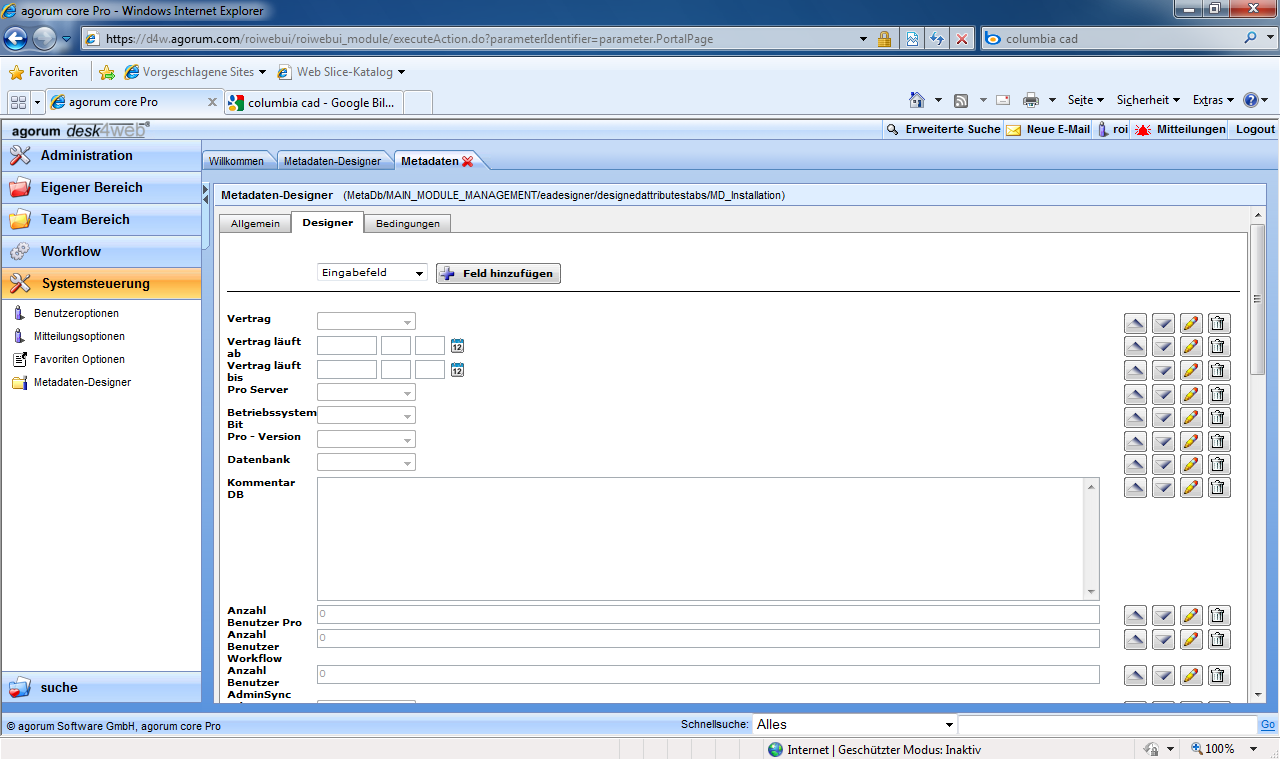
\includegraphics[width=16cm]{Bilder/agorum-core-metadatendesigner.png}
\caption{Metadaten Designer von "`agorum core"' im Web-Interface}
\label{metadatendesigner agorum}
\centering
\end{figure}

Das Einlesen und Bereitstellen von Dokumenten in "`agorum core"' funktioniert schon mit der freien Version. Jedoch kann hier nur eine Standard Suche und Ablage verwendet werden. \cite{agorum_preise}

Das automatische erkennen von Standard-Metadaten in Dateien funktioniert, jedoch auch nur mit der entsprechenden "`Pro"'-Version oder einer Zubuchung genau wie die Versionierung von Dateien.

"`agorum core"' verf\"ugt \"uber verschiedene Schnittstellen, welche von Frontends angesprochen werden k\"onnen. 

\subsection{Alfresco}
\subsection{Open Xchange}
% \subsection{anderes ECM}
\subsection{Auswertung der M\"oglichkeiten}\label{Auswertung ECM}
\textcolor{green}{\checkmark} \textcolor{red}{X} \textcolor{orange}{\checkmark X}